\documentclass[tikz,border=5pt]{standalone}
\usepackage[UTF8]{ctex}
\usepackage{amsmath,amssymb}
\usetikzlibrary{arrows.meta,calc,angles,quotes,patterns,decorations.pathmorphing}
\definecolor{field}{HTML}{176B9B}
\definecolor{force}{HTML}{B64B32}
\tikzset{>=Latex,line width=.8pt,every node/.style={font=\small},field/.style={color=field},force/.style={color=force},body/.style={draw=black,fill=blue!6},ghost/.style={dashed,gray},labelbox/.style={fill=white,inner sep=1.5pt}}
\begin{document}
\begin{tikzpicture}
\draw[->](-3,0)--(3.5,0)node[right]{$x$};
\draw[body](-1.7,0)circle(.22)node[below=8pt]{$m$};
\draw[body](.2,0)circle(.22)node[below=8pt]{$m$};
\draw[->,field](-1.7,.5)--(-.55,.5)node[midway,above]{$u_1$};
\draw[->,field](.2,.5)--(.9,.5)node[midway,above]{$u_2$};
\node[below,align=center]at(0,-1){有符号初速度沿同一直线\\散射后的速度可进入空间方向};
\end{tikzpicture}
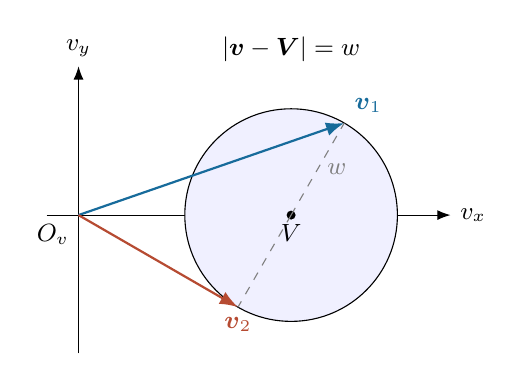
\begin{tikzpicture}[scale=1.35]
\draw[->](-.3,0)--(3.5,0)node[right]{$v_x$};
\draw[->](0,-1.3)--(0,1.4)node[above]{$v_y$};
\draw[body](2,0)circle(1);
\fill(2,0)circle(1.2pt)node[below]{$V$};
\draw[->,field,thick](0,0)--(2.5,.866)node[above right]{$\boldsymbol v_1$};
\draw[->,force,thick](0,0)--(1.5,-.866)node[below]{$\boldsymbol v_2$};
\draw[ghost](2,0)--(2.5,.866)node[midway,right]{$w$};
\draw[ghost](2,0)--(1.5,-.866);
\node[below left]at(0,0){$O_v$};
\node[above]at(2,1.35){$|\boldsymbol v-\boldsymbol V|=w$};
\end{tikzpicture}
\begin{tikzpicture}
\begin{scope}
\draw[->](0,0)--(3.3,0);
\draw[->,field](0,0)--(2.5,.866)node[above]{$\sqrt7\,u$};
\draw[->,force](0,0)--(1.5,-.866)node[below]{$\sqrt3\,u$};
\draw (.7,0)arc(0:19.1:.7);
\draw (.95,0)arc(0:-30:.95);
\node[right]at(.8,.28){$19.1^\circ$};
\node[right]at(1.1,-.35){$30^\circ$};
\node[above]at(1.5,1.4){同向初速度 $3u,u$};
\end{scope}
\begin{scope}[xshift=5.7cm]
\draw[->](-.3,0)--(3,0);
\draw[->,field](0,0)--(2,1.732)node[above]{$\sqrt7\,u$};
\draw[->,force](0,0)--(0,-1.732)node[below]{$\sqrt3\,u$};
\draw(.7,0)arc(0:40.9:.7);
\node[right]at(.9,.6){$40.9^\circ$};
\draw(.25,0)--(.25,-.25)--(0,-.25);
\node[above]at(1.5,2.1){反向初速度 $3u,-u$};
\end{scope}
\end{tikzpicture}
\end{document}
